\chapter{Tutorial}
\label{c:tutorial}

This chapter gives a brief tutorial of \tao to get you, the user, up
and running with \tao without needing to dredge through the entire
reference manual. See Chapter~\sref{c:concepts} for a discussion of
\tao terminology.

%----------------------------------------------------------------
\section{Obtaining Tao}
\label{s:obtaining}

Instructions for setting up the appropriate environmental variables
and for obtaining the source files can be found at:
\begin{example}
  http://www.lepp.cornell.edu/~dcs/bmad/
\end{example}

Briefly, you should be able to run \tao using the command
\begin{example}
  \$ACC_EXE/tao \{-init <tao_input_file>\} \{-beam_all <beam_file>\} 
           \{-beam0 <beam_file>\} \{-lat <lattice_file>\}
\end{example}
\vn{\$ACC_EXE} is an environmental variable pointing to the directory
the \tao executable is in.  The root initialization file
\vn{<tao_input_file>} is the file that \tao reads to start \tao's
initialization process. If not present, \vn{<tao_input_file>} defaults
to \vn{tao.init}. The \vn{-beam_all} switch is for reading in data
generated from beam tracking (\sref{s:beam.init}). The \vn{-beam0}
switch is for specifying the initial beam distribution.  The
\vn{-lat} switch is used to override the lattice file specified in
the root initialization file. See section~\sref{s:command.line} for
more details. Example:
\begin{example}
  \$ACC_EXE/tao -init my.init -lat xsif::slac.xsif
\end{example}
An initialization file is actually not needed. In this case, a
\vn{-lat} switch is manditory and \tao will use a set of default plot
templates for plotting.

This tutorial uses the example set of input files that comes with the \tao library.
These files can be viewd and/or downloaded at:
\begin{example}
  https://accserv.lepp.cornell.edu/cgi-bin/view.cgi/trunk/src/tao/program
\end{example}
On a unix machine with the Subversion \vn{svn} client program, 
these files can be obtained more simply via the command:
\begin{example}
  svn co https://accserv.lepp.cornell.edu/svn/trunk/src/tao/program
\end{example}
this will create a sub-directory \vn{program} of your current directory with 
the appropriate files.

%----------------------------------------------------------------
\section{Initializing Tao}
\index{initializing!files}
\label{s:initializing}

Initialization occurs when \tao is started. The initialization
information can reside in one file or it can be split into a number of
files as discussed in Section~\sref{s:init.global}.

Using the example files provided with \tao (\sref{s:obtaining}), \tao
is started with the command:
\begin{example}
  \$ACC_EXE/tao
\end{example}
Since no initialization file is specified on the command line, the
default file \vn{tao.init} is used. In the example \vn{tao.init} there
is the following:
\begin{example}
  &tao_start
    plot_file = 'tao_plot.init'
  /
\end{example}
The plotting information will
come from the file \vn{tao_plot.init}. Since no other initialization
files are specified (\sref{s:init.global}), \tao will look for the
non-plotting information (except for the lattice file) in \vn{tao.init}.

The lattice file is specified in the \vn{tao_design_lattice} namelist
in \vn{tao.init}:
\begin{example}
  &tao_design_lattice
    n_universes = 1
    design_lattice(1) = "bmad_L9A18A000-_MOVEREC.lat"
  /
\end{example}
\tao will setup a single universe since \vn{n_universes = 1}.
By default, \tao assumes that this lattice uses the \bmad lattice
format.  With the above information, \tao has the information on what
files it needs to read to initialize itself.

%----------------------------------------------------------------
\section{Getting information from Tao}
\label{s:get.info}

%----------------------------------------------------------------
\subsection{The Plotting Window}\index{plotting}

When \tao first starts up, \tao will create a new window for
displaying plots. This window will be called the \vn{plot}
window. Commands to \tao can be typed in from the original window from
which \tao was invoked. This will be called the \vn{command} window.

As a first step, let us command \tao to display some plotting
information using the command:
\begin{example}
  show plot
\end{example}
The information will be displayed in the command window. The first
section of the \vn{show plot} output shows information on font sizes:
\begin{example}
  plot_page parameters:
  %size                       =   4.00000000E+02  5.00000000E+02
  %n_curve_pts                =      401
  %text_height                = 12.000
  %main_title_text_scale      = 1.300
  %graph_title_text_scale     = 1.100
  %axis_number_text_scale     = 0.900
  %axis_label_text_scale      = 1.000
  %key_table_text_scale       = 0.900
  %legend_text_scale          = 0.800
  %shape_height_max           = 40.000
\end{example}
See section~\sref{s:init.plot} for more details. 

The second section of the \vn{show plot} output
lists the plot \vn{templates} (\sref{s:plotting}) and
\sref{s:template}) that \tao knows about:
\begin{example}
 Templates:
   Plot                .Graph
   ------------------  ----------
   orbit               .x  .y
   phase               .a  .b
   beta                .a  .b
   eta                 .x  .y
   cbar                .22  .12  .11
   quad_k1             .k1
   floor               .this
\end{example}
In this case, these templates are defined in the \vn{tao_plot.init}
file. There is an \vn{orbit} plot template which has two associated
graphs: \vn{orbit.x} and \vn{orbit.y}, etc. To see more information on, for example,
the \vn{phase} template plot, use the command
\begin{example}
  show plot phase
\end{example}
and to see more information on, for example, the \vn{orbit.y} graph use the command
\begin{example}
  show plot orbit.y
\end{example}
Similarly, the \vn{show plot} command can be used to display
information about the curves within each graph.

The next block of information in the \vn{show plot} command is:
\begin{example}
Visible  Plot Region         <-->  Template             x1    x2    y1    y2
-------  -----------               -----------------------------------------
   T     top                 <-->  orbit               0.00  1.00  0.48  0.95
   T     bottom              <-->  phase               0.00  1.00  0.00  0.48
\end{example}
This shows that two plot regions have been defined called \vn{top} and
\vn{bottom}. Each region contains a visible plot and the plot template
associated with the \vn{top} region is the \vn{orbit} template, etc.

Figure~\ref{f:plot.begin} shows what you will see in the plot
window. In the top two plots you see the \vn{x} and \vn{y} model
lattice orbit data. The horizontal axis is the \cesr BPM index. The
horizontal pretzel and L03 vertical bump in CESR can be clearly
seen. The slight vertical displacement due to the solenoid
compensation can also be seen around the IP. The orbit data is for a
closed orbit electron (this being a storage ring). The bottom two
plots show the relative particle phase, that is, the difference
between the model and design phases (as documented in the plot title
as [model - design]). Two plot regions are defined in \tao
\vn{top} and \vn{bottom}.

\index{commands!plot}
As a first step let's view the absolute model phase. Use the command:
\begin{example}
  plot bottom model
\end{example}
This will change the data plotted in the bottom two graphs to just the
model.  The plots are now way off scale. Let \tao automatically set
the scale by typing:
\index{commands!scale}
\begin{example}
  scale bottom
\end{example}
As expected, the phase increases approximately linearly as the
particle travels through the ring. Zero phase is halfway through the
ring (at L03 in \cesr lingo).  This is always true. Absolute phase is
arbitrary so \tao sets the average phase to zero when generating the
data. To set this back to relative phase type:
\begin{example}
  plot bottom model - design
\end{example}

Let's now look at the beta function by typing
\index{commands!place}
\begin{example}
  place bottom beta
\end{example}
Again, we need to rescale the plots by typing
\index{commands!scale}
\begin{example}
  scale bottom
\end{example}
We see the periodic FODO beta function where large horizontal beta
corresponds to small vertical beta and vice versa.

Likewise, we can look at the dispersion in the top two graphs by
typing
\index{commands!scale}
\begin{example}
  place top eta
  scale top
\end{example}
The plot window should now look like Figure~\ref{f:plot.eta.beta}.

Now let's look at the coupling (C-matrix) by typing
\begin{example}
  place bottom cbar
  scale bottom
\end{example}
We see that there is strong coupling within the CLEO solenoid and
virtually no coupling anywhere else. To zoom in the scale so that we
can see the residual coupling outside the interaction region type
\begin{example}
  scale bottom -0.01 0.01
\end{example}
The \vn{**Limited**} displayed in red on the bottom plots tells us
that there are data points outside the plotted region.  We now see
that there is a small amount of coupling at the L03 region (BPM
indexes 45-55) and a few other places along the ring. Your plot window
should now look like Figure~\ref{f:plot.coupling.no.IR}.

The x-axis is currently the BPM index number. It is sometimes
convenient to plot the data versus longitudinal position. This is done
by typing
\index{commands!x-axis}
\begin{example}
  x-axis * s
\end{example}

The \cmd{all} will apply the change to all plot areas (both top and
bottom). In any of the above commands \cmd{top} or \cmd{bottom} could
have been replaced with \cmd{all}.

Variables can also be plotted provided the proper plot template has
been set up in the plot initialization file (See
Section~\sref{s:init.plot} for details on initializing plotting). Type
the following to view the quadrupole k1 values:
\begin{example}
  place bottom quad_k1
\end{example}
\index{commands!plot}
\index{commands!place}

\begin{figure}
  \centering
  \includegraphics[width=5in]{plot-page1.eps}
  \caption{The plot window at startup}
  \label{f:plot.begin}
\end{figure}

\begin{figure}
  \centering
  \includegraphics[width=5in]{plot-eta-beta.eps}
  \caption{Plotting dispersion and beta function}
  \label{f:plot.eta.beta}
\end{figure}

\begin{figure}
  \centering
  \includegraphics[width=5in]{plot-coupling-no-IR.eps}
  \caption{Zooming in on the residual coupling outside the IR.}
  \label{f:plot.coupling.no.IR}
\end{figure}

%----------------------------------------------------------------
\subsection{The Show Command}

Anything in the super-universe can be displayed using the \cmd{show}
command (\sref{s:show}). To get a list of the data elements currently
defined in \tao type
\index{commands!show}
\begin{example}
  show data
\end{example}
the output should look like:
\begin{example}
  Name                                   Using for Optimization

  orbit.x[0:99]
  orbit.y[0:99]

  phase.a[0:99]
  phase.b[0:99]

  eta.x[0:99]
  eta.y[0:99]

  beta.a[0:99]
  beta.b[0:99]

  cbar.11[0:99]
  cbar.12[0:99]
  cbar.21[0:99]
  cbar.22[0:99]

  k.11b[0:99]
  k.12a[0:99]
  k.12b[0:99]
  k.22a[0:99]
\end{example}
There are six \vn{d2} data types (\sref{s:data.org}) defined in the
initialization file: \vn{orbit}, \vn{phase}, etc.  The \vn{beta} data is further
subdivided into two \vn{d1} data arrays labeled \vn{beta.a} and \vn{beta.b}.
Each of these arrays has 100 data points indexed from 0 to 99.

The \vn{``Using for Optimization''} column is blank indicating that no data
would be used in an optimization (\sref{c:opti}).

To see the data values for the horizontal beta function for \cesr BPMs
1 through 50 type
\begin{example}
  show data beta.a[1:50]
\end{example}
Since we haven't changed any elements in the lattice yet the model
values equal the design values. Also note that \vn{beta.a} is actually
the a-mode betatron function. In regions with little or no coupling,
the a-mode is almost completely in the horizontal plane.

A significant point: The convention in \bmad is to label the twiss
parameters as \vn{x} and \vn{y} but they are actually the \vn{a} and
\vn{b} normal modes. So in regions of strong coupling \vn{beta.a} does
not correspond to \vn{orbit.x} which is always in the true horizontal
lab frame.  However, if you wish, you can re-label your twiss data
planes as \vn{a} and \vn{b}.  Section~\ref{c:init} shows you how to do
this. Keep in mind that lattice twiss parameters are defined
\textit{only for uncoupled betatron motion} so this is all that is
provided as data types for single particle tracking.  However, true
lab-frame \vn{x} and \vn{y} twiss parameters can be defined for a
distribution of particles so for beam
tracking true lab-frame \vn{x} and \vn{y} twiss parameters can be
calculated and are provided as data types for those tracking
types. See the \bmad manual for how to convert from normal mode
coordinates to lab-frame coordinates.

This tutorial uses single particle tracking and the twiss parameters
are found about the orbit of the tracked particle. There is another
tracking type called particle beam tracking. This
tracking type will not be explored in this tutorial.

You can also view variables by typing
\begin{example}
  show var
\end{example}
To view the quadrupole k1 values for \cesr quadrupoles 5 and 20
through 30 type
\begin{example}
  sho var quad\_k1[5,20:30]
\end{example}
Again, since we haven't changed any quadrupoles the model values are
all at their design values.

You can also see the details of a particular lattice element. To view
the details for quadrupole Q05W type
\begin{example}
  sho ele Q05W
\end{example}

\vn{show var} and \vn{show ele} show two completely different types of
structures in \tao. Elements are the actual lattice elements as known
to \bmad.  Variables are native \tao structures that act kind of like
\bmad \textit{overlays} and only indirectly control the lattice
elements.

A list of lattice elements between two elements can be shown by typing 
\begin{example}
  sho lattice 0:20
\end{example}
This will show a list of all the lattice elements between and
including elements 0 and 20. Twiss parameters and orbit information, at
the exit end of each element, is also shown.

Anything printed to the display using the \vn{show} command can also
be printed to a file by typing
\begin{example}
  show -write <file_name> <what_to_show>
\end{example}
\index{commands!show}

A list of all intrinsic \vn{tao} commands can be found by typing
\index{commands!help}
\begin{example}
  help
\end{example}
This will not list any custom commands. Detailed help on any
individual command can be found with
\begin{example}
  help <command\_name>
\end{example}
where \vn{<command_name>} is the command you want help with.

%----------------------------------------------------------------
%----------------------------------------------------------------
\section{Modifying the Lattice}
\label{s:modify.lattice}

%----------------------------------------------------------------
\subsection{Changing a Variable}
\label{ss:change.variable}

Let's change a variable and see what happens to the lattice. We are going to
change a quadrupole strength so we should plot the change in beta and phase.
Type the following (everything after the `!' are just comments and can be
omitted):
\begin{example}
  x-axis * index        ! let the data index be the x-axis
  place top beta          ! plot Beta data on top plot
  place bottom phase      ! plot phase data on bottom plot
  plot * model - design ! plot the difference between model and design data
  scale                   ! scale all plots
\end{example}

The k1 value can be increased by 0.01 units for quadrupole Q05W by typing
\index{commands!change}
\begin{example}
  change var quad\_k1[5] 0.01
  scale
\end{example}
Note the information returned on the command line after the command
and the relative changes in beta and phase in the plot window. This is
a vertically focusing quadrupole so the vertical beta and phase are
affected more than the horizontal. The \cmd{0.01} at the end of the
command tells \tao to change this variable by 0.01 units. If you want
to set a variable to a particular value then use a ``@'' before the
value. So, to change this quadrupole k1 to -0.348 type
\begin{example}
  change var quad\_k1[5] @-0.348
\end{example}

%----------------------------------------------------------------
\subsection{Putting things back where you found them}
\label{ss:put_it_back}

Let's put this quadrupole back where we found it. We can also modify
the quadrupole by modifying the lattice element directly by typing
\begin{example}
  change ele Q05W k1 d0.0
\end{example}
By modifying the element directly with the \cmd{change ele} command
you can modify almost any attribute of the element listed in the
output of \cmd{show ele Q05W}.  The ``d'' before the value is used to
set the variable relative to the design value.
\index{commands!change}

If you've changed the lattice around a lot using variables, a great
way to set all variables back to their design values is to type
\index{commands!set}
\begin{example}
  set var *|model = *|design
\end{example}
This only works if you just changed variables. If you changed any
elements directly with the \cmd{change ele} command then this will not
work. To set every attribute of every element back to the design type
\begin{example}
  set lattice model = design
\end{example}
Note that this will also recalculate the data and variable values
associated with the the model lattice to reflect the change so all the
bookkeeping is done for you.


%----------------------------------------------------------------
%----------------------------------------------------------------
\section{Using the Optimizer for Lattice Correction and Design}
\index{optimization}
\label{s:optimizer}

\index{lm!optimizer}\index{de!optimizer}
There are three non-linear optimizers included with \tao: Two
optimizers are based on the Levenburg-Marquardt method. These are
referred to as `\vn{lm}', and \vn{lmdif}', the third optimizer is
based upon \vn{Differential Evolution} and is called `\vn{de}'. This example
will use the Levenburg-Marquardt optimizer which first uses steepest
decent to zero in on the region containing the minimum then uses the
inverse-Hessian to converge on the minimum. See Numerical Recipes in
Fortran (or C or C++) for a detailed explanation. There's no need to
know the details in order to use either optimizer. Once you set up the
problem \tao has the proper wrapper routines to do the
optimization. Of course, you are not limited to using the included
optimizers. Custom analysis can be done using custom routines but
these two optimizers have been integrated `out of the box' with the
\tao data and variable structures to make quick optimization possible.

Basically, the `\vn{lm}' is typically faster since it uses a Jacobian
or ``dmerit'' matrix to find the data derivatives versus each variable
before starting the optimization process.  However it assumes the
second derivative is fairly smooth, so for very complex function
spaces the `\vn{de}' may work better. But because `\vn{lm}' typically
converges much faster (for functions it can handle) it is recommended
to try this one first and only use `\vn{de}' if it fails.

%----------------------------------------------------------------
\subsection{Fix a Messed Up lattice}
\label{ss:fix_it}

Let's mess the lattice up a little and see if the optimizer can
``fix'' the lattice. First transfer the ``correct'' or \vn{design}
lattice to the \vn{meas} data area.
\begin{example}
  set data *.*|meas = *.*|design
\end{example}
Now mess up the lattice a bit. We'll be messing with quadrupoles so
plot beta and phase.
\begin{example}
  place top beta
  place bottom phase
  plot * meas - model
  change var quad\_k1[10] 0.001
  change var quad\_k1[21] -0.001
  change var quad\_k1[67] -0.005
  scale
\end{example}
The lattice is now sufficiently screwed up.

Now specify what variables and data to use in the optimization. First type
\begin{example}
  show top10
\end{example}
to see what data is effecting the merit function the most. The merit
function is defined by
\Begineq
  {\cal M} \equiv \sum_{i} w_i \,
    \bigl[ \data_\model(i) -  \data_\meas(i) \bigr]^2 + 
  \sum_{j} w_j \,
    \bigl[ \var_\model(j) - \var_\meas(j) \bigr]^2
  \label{eq:merit}
\Endeq
where $w_{i}$ and $w_{j}$ are the weights given to each component.
The optimizer tries to minimize the merit function by changing the
model to look like the measured data. From the \vn{top10} output we
see that the beta function is effecting the merit function the
most. Since we are looking at beta and phase let's only use that data
in the optimization.
\begin{example}
  veto data *         ! Veto all the data
  use  data beta      ! Use all the beta data
  use  data phase     ! And use all the phase data
\end{example}
We also know that we need to change quadrupoles to correct the lattice.
\begin{example}
  veto var *           ! veto all the variables
  restore var quad\_k1 ! restore just the quad\_k1 variables
\end{example}
Note that we need to specify what data and variables we will be using
beforehand in the initialization files. This is already taken care of
in the demo initialization files. You can view these files to see how
the data and variables were initialized. Raw lattice elements cannot
be used by the included optimizer but there is no such restriction on
custom optimizers.

Now let's see if we have the optimizer set up correctly.
\begin{example}
  sho optimizer
\end{example}
Whoops! we want to use the Levenburg - Marquardt optimizer so
\begin{example}
  set global optimizer = lm
  show opti
\end{example}
The second command is short-hand. Most \tao commands can be shortened
to the least number of characters needed to distinguish the command
from all others.

Now we're ready to run the optimizer or ``fit'' the model to the
`measured' data.
\begin{example}
  run
\end{example}
You see the optimizer going through its cycles and it did it! The
model is now ``fitted.'' We can see what changes where done to the
quadrupoles by typing
\begin{example}
  sho var quad\_k1
\end{example}
The optimizer came very close to finding the ``design''
lattice. However, it changed more quadrupoles than just 10, 21 and
67. This isn't surprising. The optimizer finds the minimum of the
merit function and there are potentially many minima, or
degeneracies.  It does it's best not to get stuck in a local minimum
and as we can see by the plotted data, the minimum found is very close
-- virtually identical -- to the design lattice optics.  A good hint
as to what variables will be adjusted is the output of \cmd{show
top10}.  The top 3 derivatives were not the quadrupoles we
adjusted. Nevertheless, the final result was a darn near perfect
match!

%----------------------------------------------------------------
\subsection{Now Not Using all of the Variables}
\label{ss:fix_it_not_all}

Alternatively, we could have used only a subset of the
quadrupoles. Say we know approximately which quadrupoles should be
adjusted. We can then specify these variables ranges.
\begin{example}
  change var quad\_k1[10]   0.001
  change var quad\_k1[21]  -0.001
  change var quad\_k1[67]  -0.005
  scale
  use var quad\_k1[8:12,20:25,65:70]
  run
  show constraints
  sho var quad\_k1[8:12,20:25,65:70]
\end{example}
Different quadrupoles than the ones we initially changed were still
adjusted by the optimizer. The end result is again very close to the
design lattice.

%----------------------------------------------------------------
\subsection{Lattice Design}
\label{ss:lattice_design}

In \vn{lattice design} (\sref{s:lattice.design}) it is generally
easiest to specify constraint data using the ``\vn{single line}''
input format (\sref{s:init.data}). For example:
\begin{example}
&tao_d2_data
  d2_data%name = 'c1' 
  universe = '1'
  default_merit_type = "max"
  n_d1_data = 1
/

&tao_d1_data
  ix_d1_data = 1
  d1_data%name = 'xx'
  default_weight = 0.1
  ix_min_data = 1
  ix_max_data = 50
  data( 1) = 'beta.a'  'end_arc' 'end_lin3' 'max'    60   1.0   T
  data( 2) = 'beta.b'  'end_arc' 'end_lin3' 'max'    60   1.0   T
  data( 3) = 'beta.a'  ''        'end_lin3' 'max'    60   1.0   T
  data( 4) = 'beta.b'  ''        'end_lin3' 'max'    60   1.0   T
  data( 5) = 'alpha.a' ''        'end_lin3' 'max'   -0.6  1e3   T 
  data( 6) = 'alpha.b' ''        'end_lin3' 'max'   -0.6  1e3   T 
/
\end{example}


%----------------------------------------------------------------
%----------------------------------------------------------------
\section{Single Mode}\index{single Mode}
\label{s:single.mode}

\tao has a \vn{single mode} in which single keystrokes are interpreted
as commands. \tao can be set up so that in \vn{single mode} the
pressing of certain keys increase or decrease variables. While the
same effect can be achieved in the standard \vn{line mode}, \vn{single
mode} allows for quick adjustments of variables. See
Chapter~\sref{c:single} for more details.

%----------------------------------------------------------------
%----------------------------------------------------------------
\section{Where to go from here}
\label{s:where.to.go}

You now have an understanding of the basic abilities of \tao. After
this tutorial, Part II of the \tao Manual should be legible and
useful.  The Reference Guide will provide the details of everything
mentioned in this tutorial.  It goes into detail of setting up your
own initialization files and how to use the optimizer. It also
includes a complete command reference with command syntax.

However, you're not yet ready to customize \tao, but this is where the
true versatility of \tao lies. So, onward to the next section and
learn how to write your own custom routines to perform whatever
accelerator calculations that strikes your fancy!
